\documentclass[aspectratio=169]{beamer}

\usepackage{color}
\definecolor{airforceblue}{rgb}{0.36, 0.54, 0.66}
\definecolor{blue-green}{rgb}{0.0, 0.87, 0.87}
\definecolor{blue-violet}{rgb}{0.54, 0.17, 0.89}
\definecolor{cadet}{rgb}{0.33, 0.41, 0.47}
\definecolor{cordovan}{rgb}{0.54, 0.25, 0.27}

\mode<presentation>
{
    \usetheme{Madrid}
    \usefonttheme{professionalfonts} 
    \setbeamercolor{local structure}{fg=blue-green}
    \setbeamertemplate{itemize subitem}{\color{cordovan}$\blacktriangleright$}
}

\usepackage{multicol}
\usepackage{color}
\usepackage[utf8]{inputenc}
\usetheme{Madrid}
\usecolortheme{beaver}

\usepackage{caption}
\DeclareCaptionFormat{citation}{%
   \ifx\captioncitation\relax\relax\else
     \captioncitation\par
   \fi
   #1#2#3\par}
\newcommand*\setcaptioncitation[1]{\def\captioncitation{\textit{Source:}~#1}}
\let\captioncitation\relax
\captionsetup{format=citation,justification=centering}
\usepackage{mwe}% for example pictures
\usepackage{tikz,lmodern}
\usepackage[absolute,overlay,showboxes]{textpos}

\title{Comunicação em Datacenters}
\subtitle{Gerência de Redes}
\author[Leandro Silva, Luís Felipe] % (optional, for multiple authors)
{Leandro Souza da  Silva \\ Luís Felipe Mattos}
\institute{IC - Unicamp}


\date{ 06 de Dezembro de 2016 }
\logo{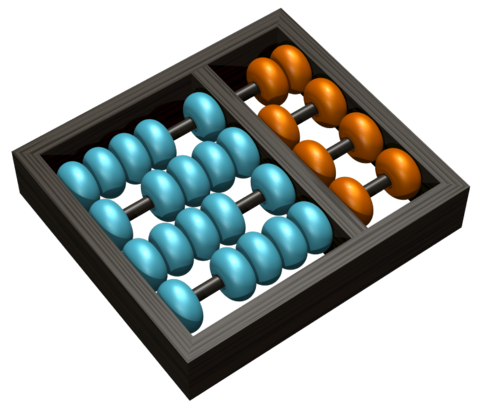
\includegraphics[height=1.0cm]{logo.png}}
 \newif\iflattersubsect
 


\AtBeginSection[] {
    \begin{frame}<beamer>
    \frametitle{Sumário} %
    \tableofcontents[currentsection]  
    \end{frame}
    \lattersubsectfalse
}

\AtBeginSubsection[] {
    \iflattersubsect
    \begin{frame}<beamer>
    \frametitle{Sumário} %
    \tableofcontents[currentsubsection]  
    \end{frame}
    \fi
    \lattersubsecttrue
}

 
\begin{document}

\begin{frame}
  \titlepage
\end{frame}

\begin{frame}{Sumário}
  \tableofcontents
  % You might wish to add the option [pausesections]
\end{frame}


\section{Introdução}

    \begin{frame} {Introdução}
        \centering
        \Large Visão Geral de um Data Center.
        \begin{figure}[ht]    
            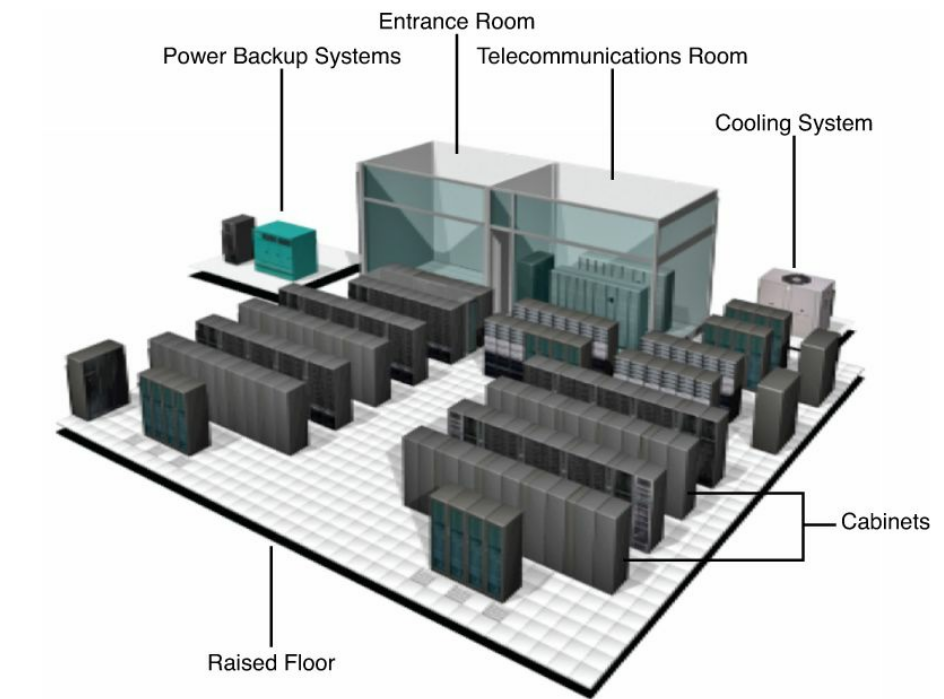
\includegraphics[scale=0.22]{datacenter.png}
            \caption{Data Center}
            \label{fig:data_center}
        \end{figure}

    \end{frame}
        
        
    \begin{frame} {Introdução}
        
         \begin{itemize}
         \setlength\itemsep{2em}
            \Large
            \item
                Com o crescimento da computação em nuvem, os datacenters passaram a receber funções novas.
                
             \item
                Certas aplicações necessitam de certos requisitos:
            \begin{itemize}
                \item
                    Escalabilidade
            
                \item
                    Tolerância a Falhas
                \item
                    Latêcia
                    
                 \item
                    Capacidade da Rede
                 \item
                    Virtualização               
            \end{itemize}
                    
         \end{itemize}
        
    \end{frame}


\section{Motivação} 

    \begin{frame} {Motivação}
            
        \centering
        \Large
             O consumo de dados pelos usuários está crescendo exponencialmente a cada ano.
            \begin{figure}[ht]    
                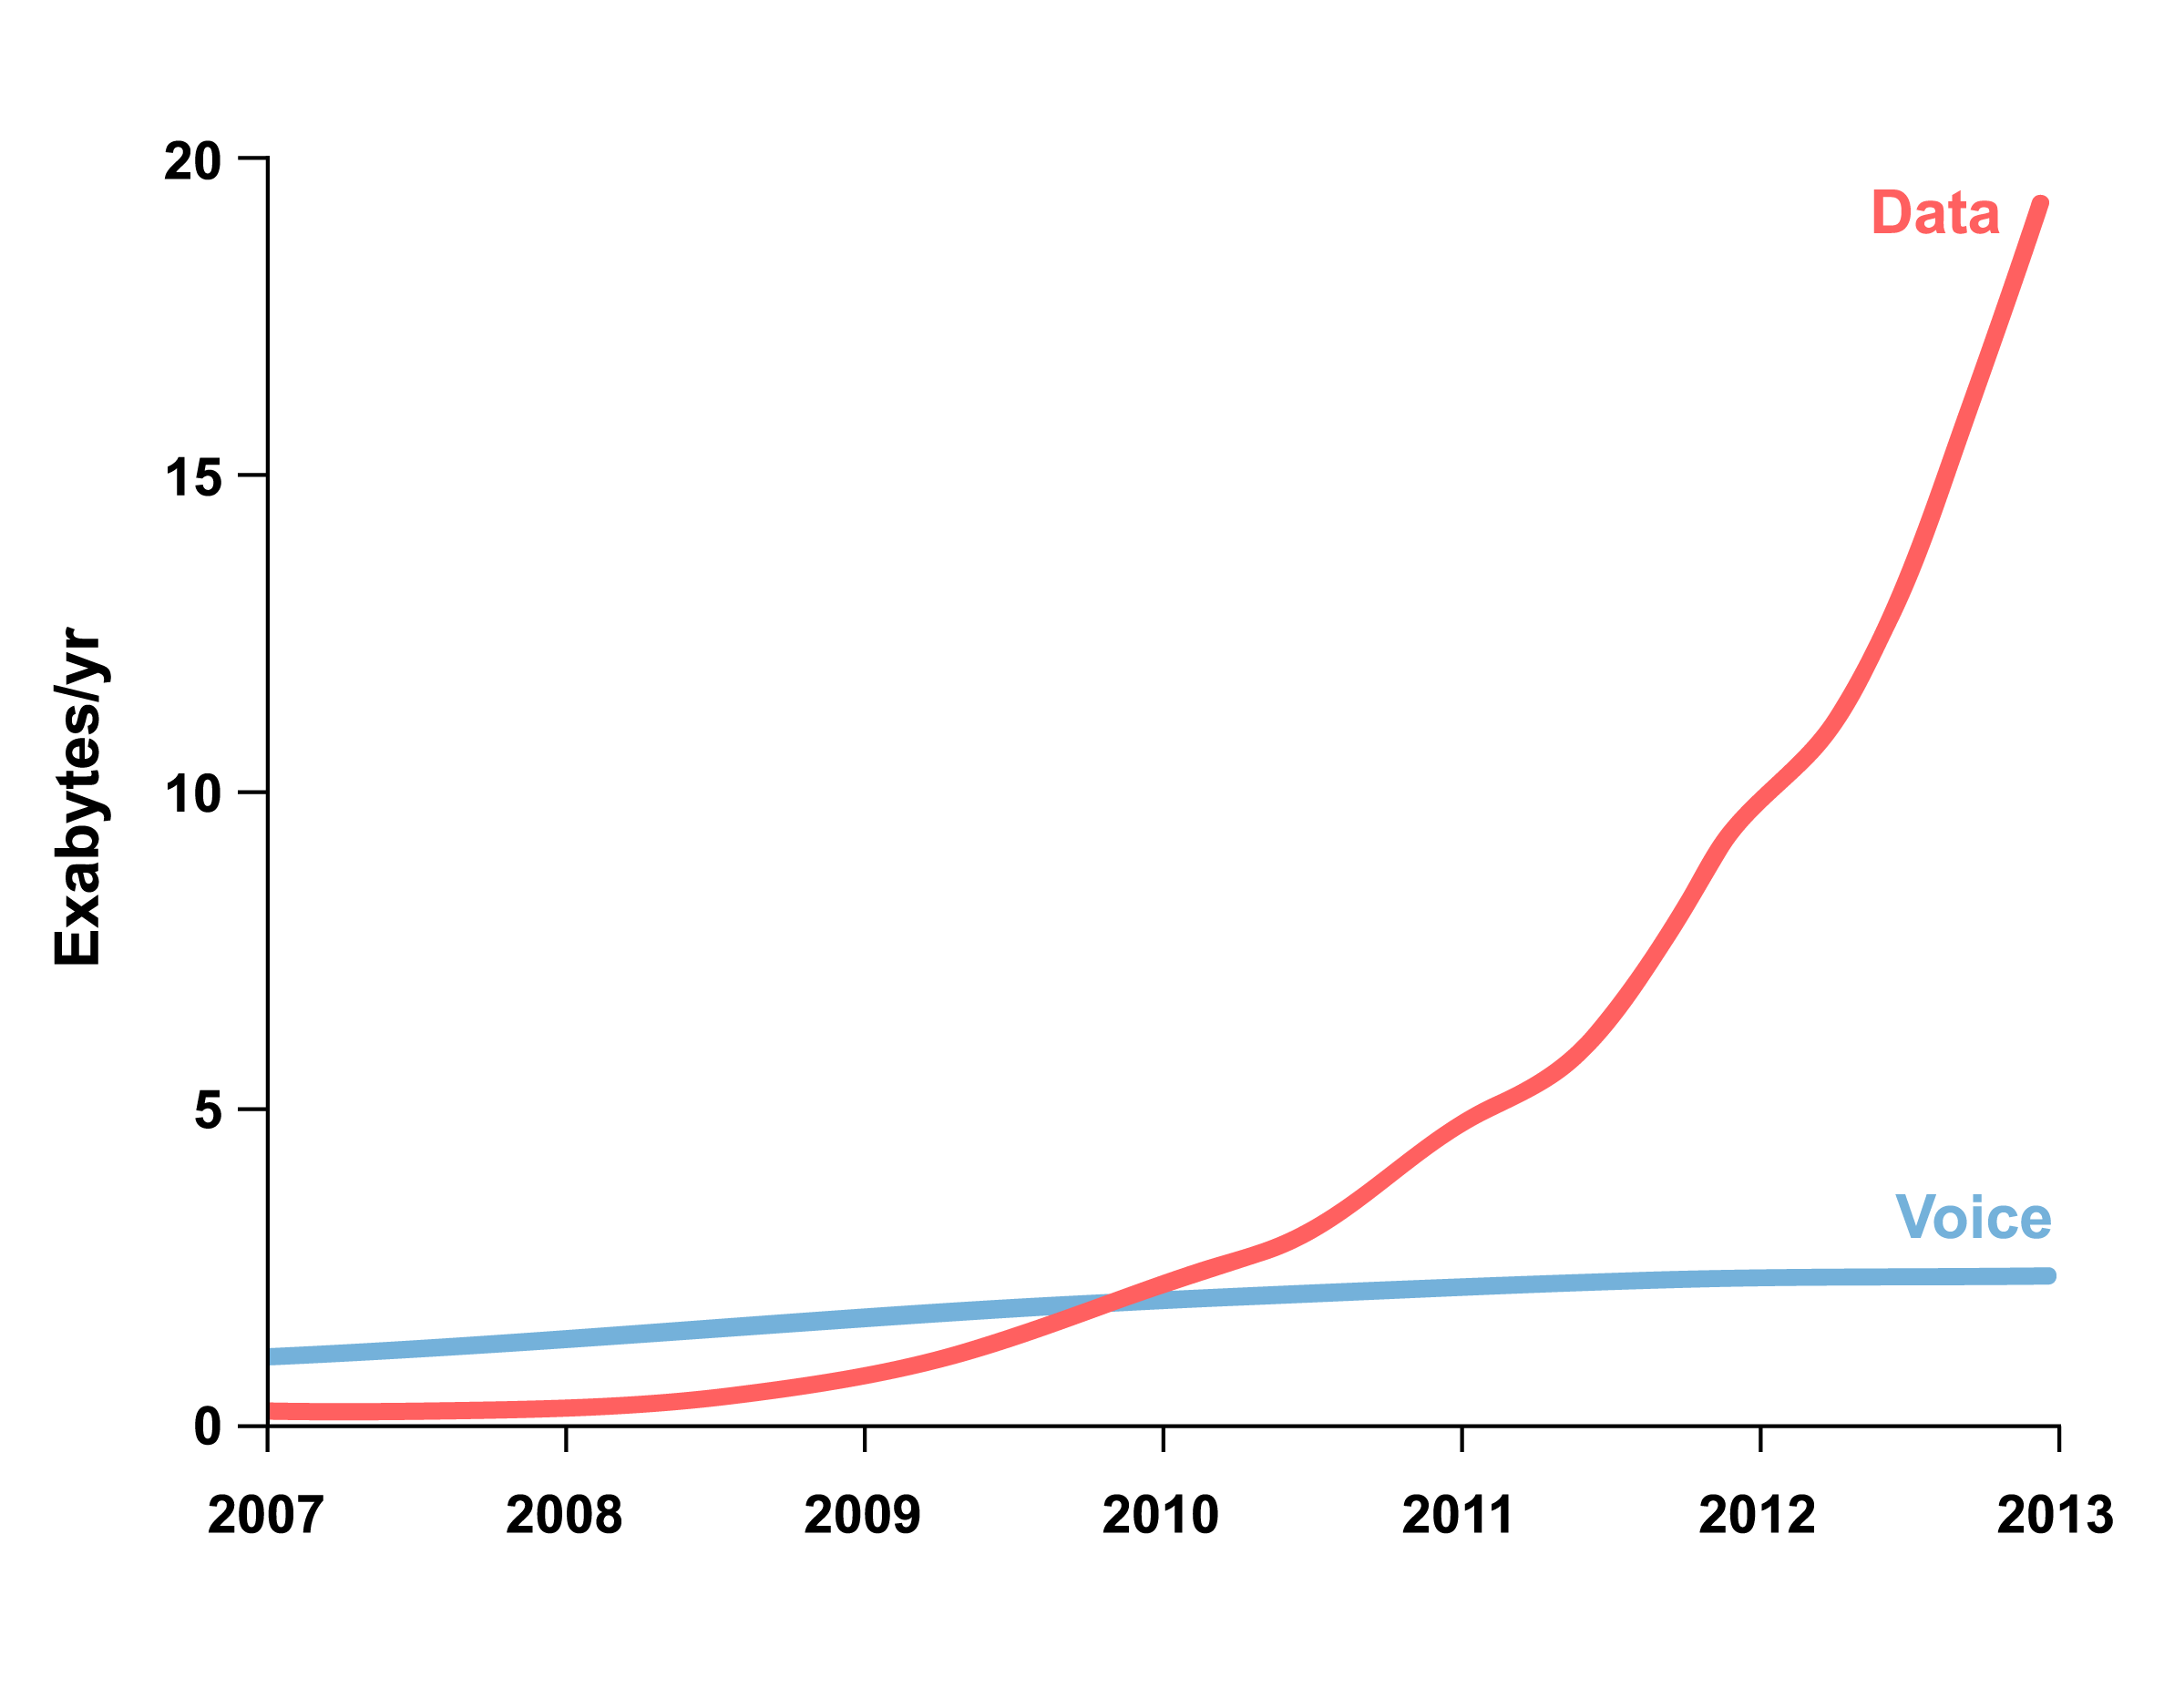
\includegraphics[scale=0.3]{consumo.png}
                \setcaptioncitation{The Cloud Begins With Coal , Ericsson Mobility Report, June 2013 }
                \caption{Consumo de dados e voz}
                \label{fig:consumo}
            \end{figure}

    \end{frame}
    
        \begin{frame} {Motivação}
            
            \centering
            \normalsize  
                Por causa disso, o número de servidores em Data Centers deve crescer exponencialmente para acompanhar a demanda, o que traz dificuldades em desenvolver redes eficientes e de baixo custo.
            \begin{figure}[ht]
       
                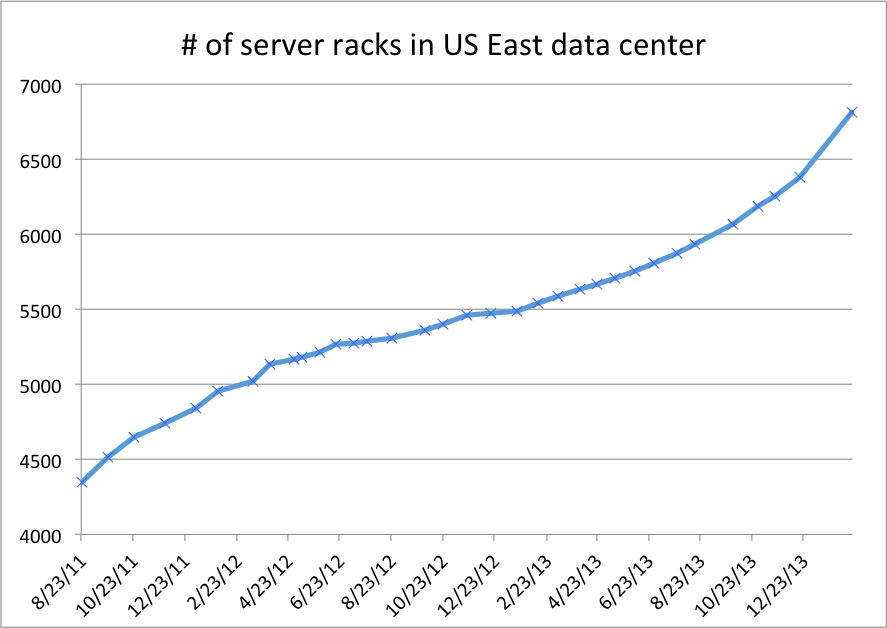
\includegraphics[scale=0.45]{servidores.png}
                \setcaptioncitation{  \href{https://huanliu.wordpress.com/category/cloud/}{https://huanliu.wordpress.com/category/cloud/ }}
                \caption{Número de servidores racks}
                \label{fig:servidores}
            \end{figure}
        
        \end{frame}
        
        \begin{frame} {Motivação}
                
            \Large
            Disponibilidade de dados e segurança se tornaram aplicações críticas.
            
        \end{frame}
                
            
        \begin{frame} {Motivação}
            \centering  
            \Large
            Por outro lado, a criação de novas tecnologias faz com que o custo dos componentes seja cada vez menor.
            \begin{figure}[ht]    
                            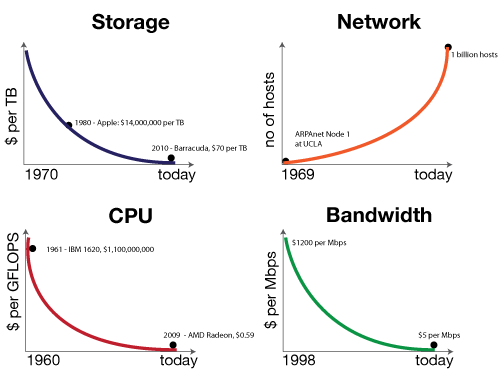
\includegraphics[scale=0.35]{custo.png}
                            \setcaptioncitation{  \href{http://radar.oreilly.com/2011/08/building-data-startups.html}{http://radar.oreilly.com/2011/08/building-data-startups.html }}
                            \caption{Custo de tecnologias}
                            \label{fig:custo}
                        \end{figure}
        \end{frame} 
            
        \begin{frame} {Motivação}
            \centering
            \Large
            Apesar disso, surge uma dificuldade cada vez maior de criar redes escaláveis exponencialmente sem que haja perda de eficiência.
            \begin{figure}[ht]    
                            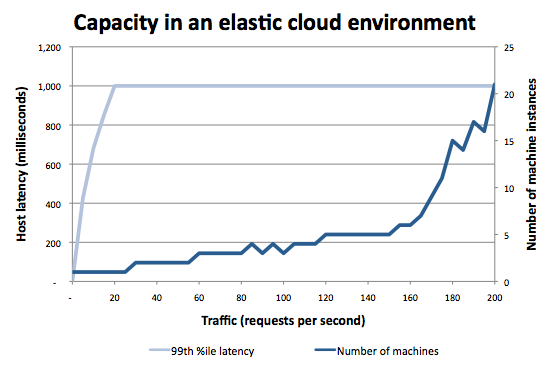
\includegraphics[scale=0.35]{capacity.png}
                             \setcaptioncitation{  \href{http://www.bitcurrent.com/the-clouds-most-important-equation/}{http://www.bitcurrent.com/the-clouds-most-important-equation/}}
                             %\href{http://tex.stackexchange.com/q/20800/5701}{\beamergotobutton{Link}}
                             \caption{Capacidade elástica em ambiente de nuvem}
                    
                            \label{fig:capacity}
                        \end{figure}
        \end{frame} 
            
        
\section{Topologias} 
    
    \subsection{Tradicionais}
    
        \begin{frame} {Topologias Tradicionais}
           \begin{columns}    
             \column{0.4\textwidth}  
             \begin{itemize}
              
             \setlength\itemsep{2em}
                \Large
                \item
                    Baseadas em ávrores.
                    
              
                \begin{itemize}
                    
                    \item
                        Basic Tree
                
                    \item
                        Fat-Tree
                
                     \item
                        VL2 
                                
                \end{itemize}
                        
             \end{itemize}
                
              \begin{itemize}
               
              \setlength\itemsep{2em}
                 \Large
                 \item
                     Recursivas.
                     
               
                 \begin{itemize}
                    
                     \item
                         Dcell
                 
                     \item
                         Bcube
                 
                      \item
                         FiConn
                                 
                       \item
                        FlatNet
                       
                       \item
                        SprintNet
                 \end{itemize}
                         
              \end{itemize}
          \end{columns} 
         \end{frame}
    
     \begin{frame} {Basic Tree}
        
        \begin{columns}    
          \column{0.7\textwidth}  
                       
            \begin{figure}[ht]    
                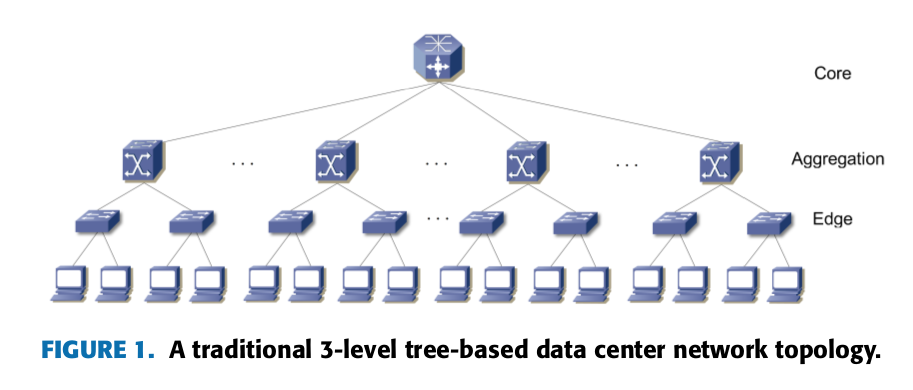
\includegraphics[scale=0.3]{basic_tree.png}
                
               
                \label{fig:consumo}
            \end{figure}
		\column{0.3\textwidth}
	
          \begin{figure}[ht]    
              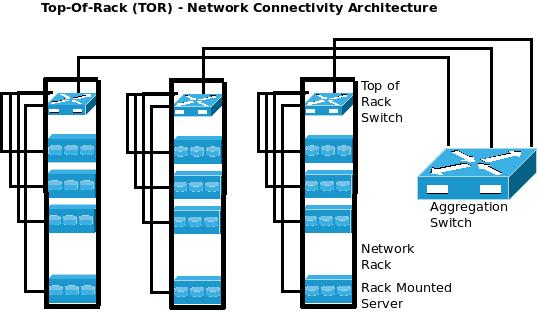
\includegraphics[scale=0.25]{imagens/tor.jpeg}
              
             
              \label{fig:consumo}
          \end{figure}
        \end{columns}
     		
     \end{frame}
     
     
     \begin{frame} {Basic Tree}
                          
          
         \Large
         \begin{itemize}
                            
          \item
                 Crescimento do Oversubscription na direção do Core da rede.
                             
          \item
              Oversubscription é a multiplexação dos recursos de banda, para economizar enlaces e equipamentos, sem reduzir o desempenho da rede.
          \item
             O Oversubscription total é a soma do Oversubscription no domínio de acesso dos servidores + Oversubscription da agregação\\
             
           
     
         \end{itemize}
            
     \end{frame}
     
     \begin{frame}
     	\Large
     	\textbf{Exemplo:}
       \begin{multicols}{2}
       		\normalsize
 					\textbf{Domínio de acesso dos servidores.}
                
                 
                        Switch 48 Portas -- 1 Gbps\\
                        20 Gbps para uplink -- servidores\\
                        Oversubscription = (48G/20G) = 2.4\\
                        1Gbps/2.4 = 416Mbps
        
       		\columnbreak
       	 
  					\textbf{Agregação}.
                 
         
                     20  Portas -- 10 Gbps\\
                     8 Para se conectar ao Core\\
                     12 Para se concetar ao switch Tor\\
                     Oversubscription = (120G/80G) = 1.5
       \end{multicols}
       		\normalsize
          Oversubscription Total = 2.4 + 1.5 = 3.9\\
               Velocidade Max de Transmissão dos Servidores = (416Mbps/1.5) = 277Mbps.
               Se Todos os servidores resolverem transmitir no máximo da capacidade da interface de 1Gbps,
               então haverá congestionamento e perda de pacotes.
     \end{frame}
     
     
     
      \begin{frame} {Fat Tree, baseada na rede CLOS}
             \begin{figure}[ht]    
                 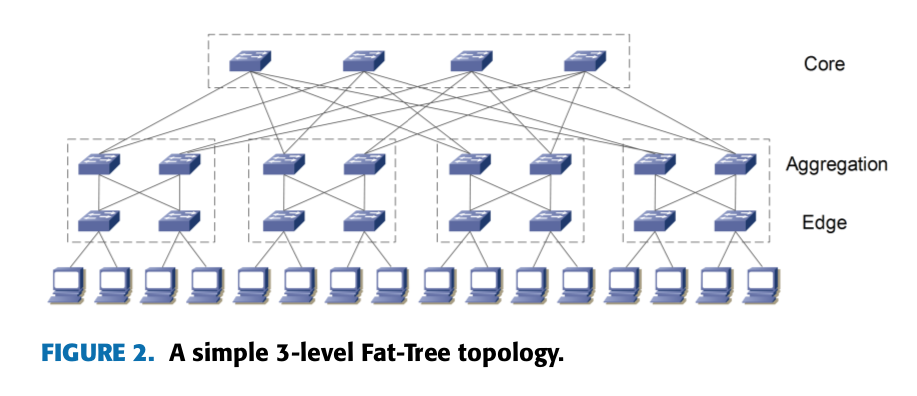
\includegraphics[scale=0.38]{fat_tree.png}
                 
                
                 \label{fig:consumo}
             \end{figure}
 
      
      \end{frame}
      

    \begin{frame} {Fat Tree, baseada na rede CLOS}
          
  	
      \Large
      \begin{itemize}
                         
       \item
              Criada por Charles Clos do MIT.
                          
       \item
          	É uma estrutura rearranjável não bloqueante.
       \item
          Fornece uma relação de Oversubscription de 1:1 a todos os servidores.
         
        \item
        	Suporta $n^3$/4 servidores, onde \textit{n} é o número de portas do switch.
       	\item
       		No entanto, a complexidade da fiação é O(n3), que é um desafio sério.
  
      \end{itemize}
         
    
    \end{frame}
      
      
      
      
       \begin{frame} {VL2}


         \begin{itemize}
             \Large
             \item
                 Switches em uma topologia de rede CLOS
         
             \item
                 Usa o VLB (Valiant Load Balancing) para distribuir tráfego entre os caminhos da rede
         
              \item
                 Usa o protocolo ARP (Address Resolution Protocol) para que seja escalável para um número grande de servidores
                         
              
         \end{itemize}
  
       
       \end{frame}
    
    	\begin{frame} {Topologias Tradicionais}
			Topologias recursivas
		\end{frame}

		\begin{frame} {Topologias Recursivas: Dcell}
			Baseada em células interligadas entre servidores
			\begin{figure}[ht]    
				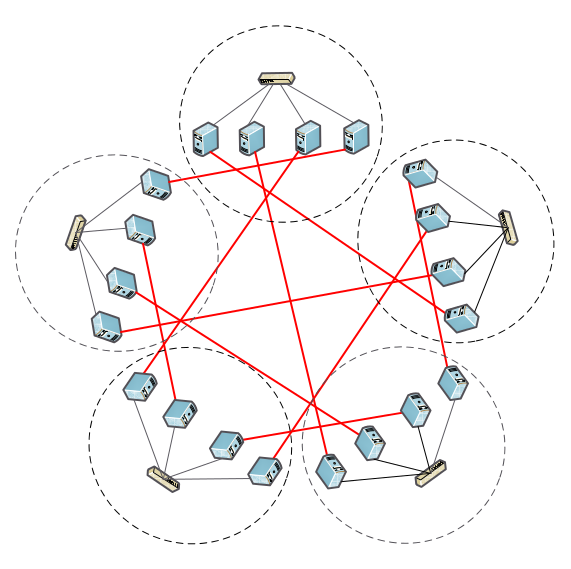
\includegraphics[scale=0.3]{imagens/dcell.png}
				\label{fig:sample_figure}
			\end{figure}
		\end{frame}

		\begin{frame} {Topologias Recursivas: Bcube}
			Baseada em células interligadas entre switches
			\begin{figure}[ht]    
				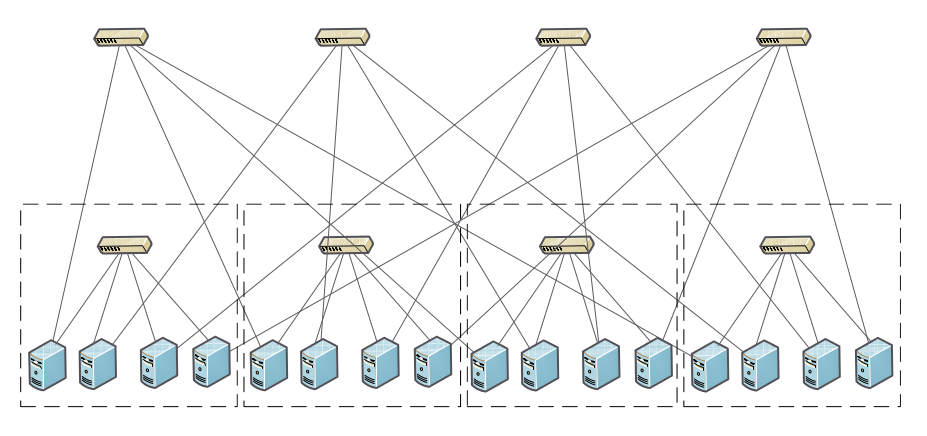
\includegraphics[scale=0.3]{imagens/bcube.png}
				\label{fig:sample_figure}
			\end{figure}
		\end{frame}

		\begin{frame} {Topologias Recursivas: FiConn}
			Semelhante à Dcell, mas o grau de cada célula é sempre 2
			\begin{figure}[ht]    
				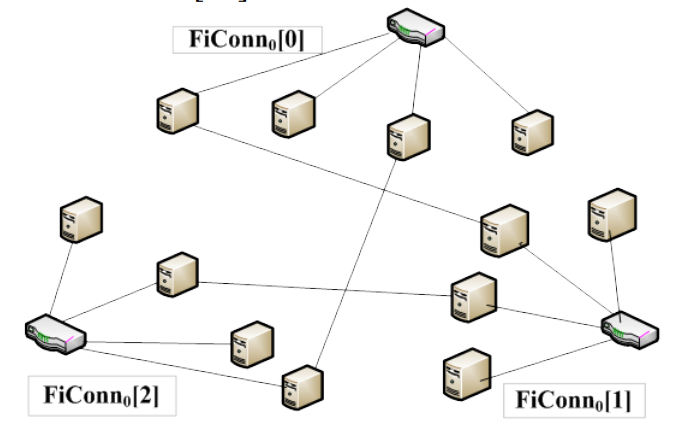
\includegraphics[scale=0.3]{imagens/ficonn.png}
				\label{fig:sample_figure}
			\end{figure}
		\end{frame}

		\begin{frame} {Topologias Recursivas: FlatNet}
			Semelhante ao BCube, porém é mais escalável
			\begin{figure}[ht]    
				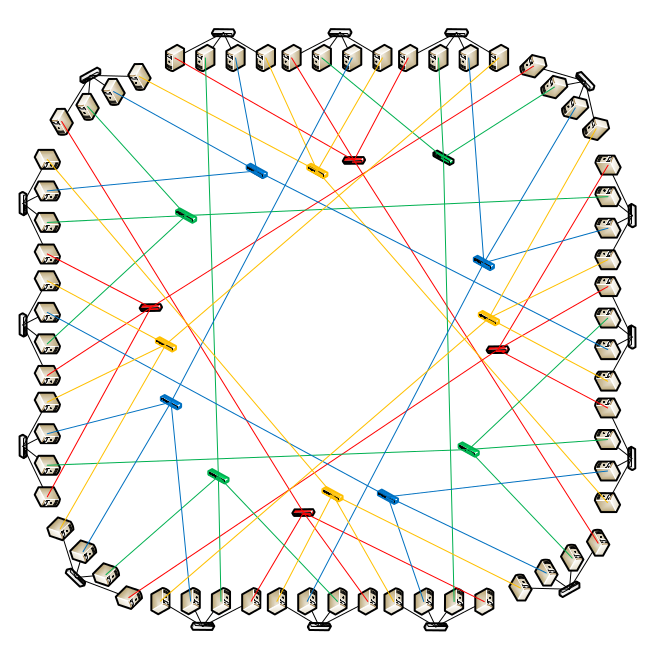
\includegraphics[scale=0.3]{imagens/flatnet.png}
				\label{fig:sample_figure}
			\end{figure}
		\end{frame}

		\begin{frame} {Topologias Recursivas: SprintNet}
			Semelhante à DCell, porém as células são compostas por 4 servidores e 2 switches de 6 portas
			\begin{figure}[ht]    
				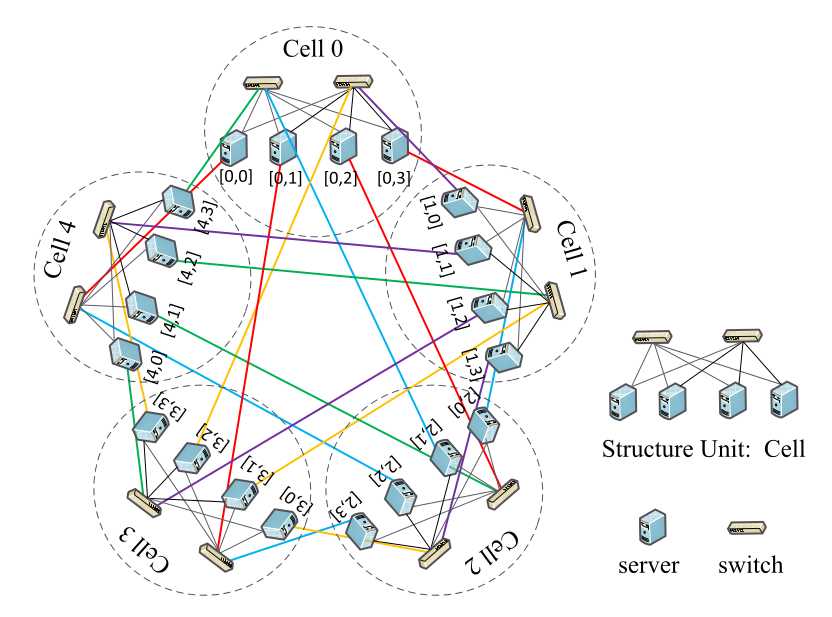
\includegraphics[scale=0.3]{imagens/springnet.png}
				\label{fig:sample_figure}
			\end{figure}
		\end{frame}

		\begin{frame} {Comparação}
			\begin{figure}[ht]   
				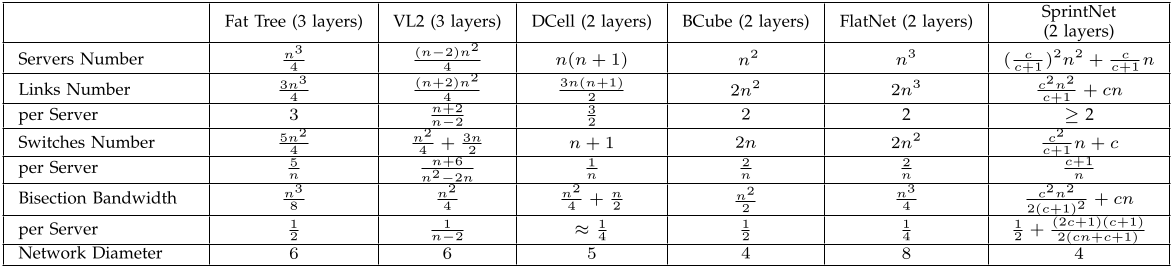
\includegraphics[scale=0.35]{imagens/tabela.png}
				\label{fig:sample_figure}
			\end{figure}
		\end{frame}

		\subsection{SDN}
		
		\begin{frame} {SDN em Datacenters}
			Com o avanço do SDN, a ideia mais básica é definir servidores virtualizados e criar uma rede virtualizada
			\begin{figure}[ht]   
				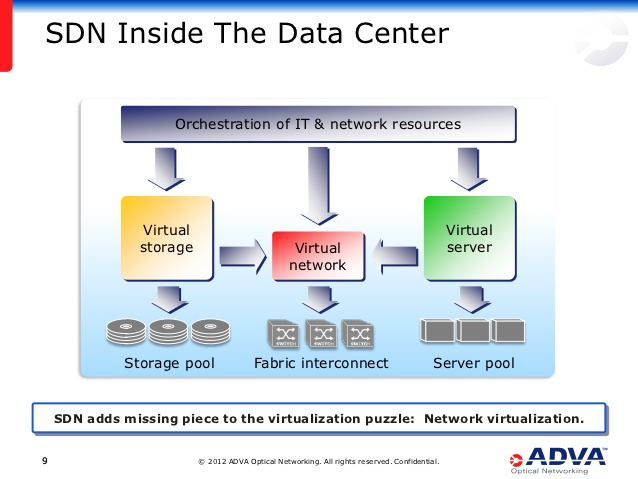
\includegraphics[scale=0.35]{imagens/inside-sdn.jpg}
				\label{fig:sample_figure}
			\end{figure}
		\end{frame}

		\begin{frame} {SDN em Datacenters}
			Esta técnica já é utilizada atualmente (PayPal por exemplo)
			\begin{figure}[ht]   
				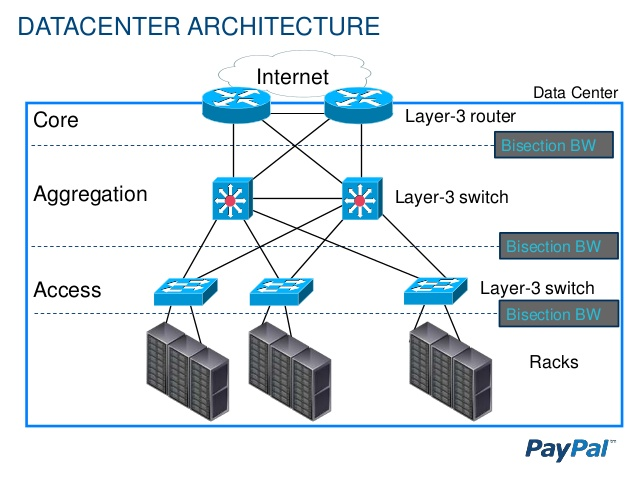
\includegraphics[scale=0.3]{imagens/sdn-1.jpg}
				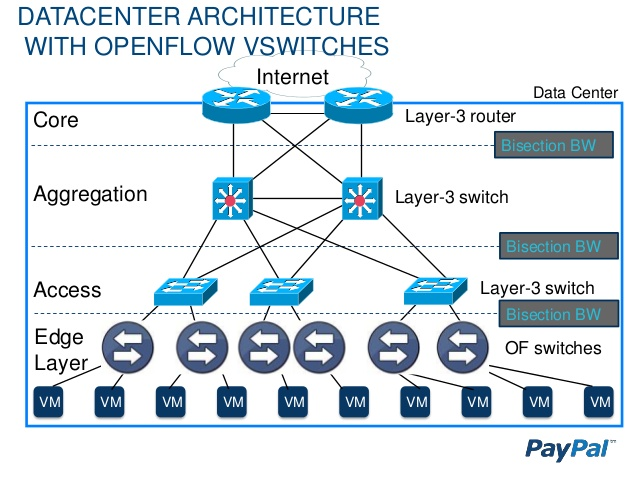
\includegraphics[scale=0.3]{imagens/sdn-2.jpg}
				\label{fig:sample_figure}
			\end{figure}
		\end{frame}

		\begin{frame} {SDN em Datacenters}
			\begin{figure}[ht]   
				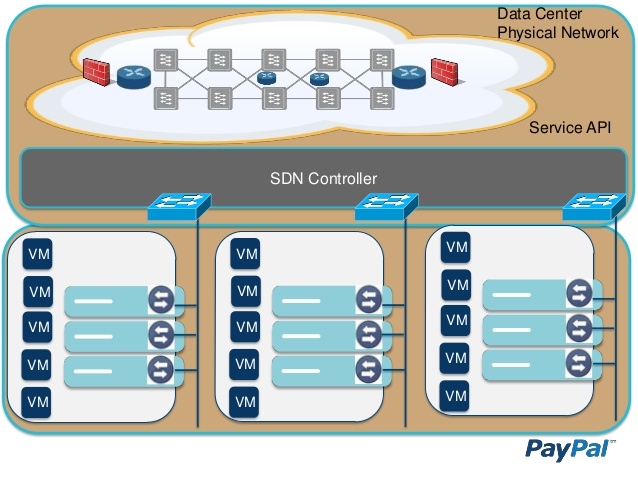
\includegraphics[scale=0.4]{imagens/sdn-3.jpg}
				\label{fig:sample_figure}
			\end{figure}
		\end{frame}


\section{Protocolos}
    \subsection{Roteamento}
    
    
    \begin{frame}{Protocolos}
    \huge
    Datacenters têm alguns requisitos básicos,  mas que causam algumas dificuldades:
   
      \begin{columns}    
        \column{0.5\textwidth}   
          \begin{itemize}
              \large            
              \item
                  RTTs precisam ser da ordem de microsegundos
          
              \item
                  Poucas multiplexações
          
               \item
                  Perda de pacotes baixa
                \item
                    Lidar com Incast
                    
               
                          
          \end{itemize}
     \column{0.5\textwidth}   
     \begin{figure}[ht]    
                     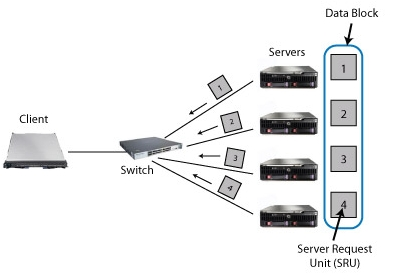
\includegraphics[scale=0.3]{problems.jpg}
                     
                    
                     \label{fig:problems}
                 \end{figure}
    
    
    \end{columns}
    
     
    
    \end{frame}
    
 
    \begin{frame} {Roteamento}
      				
                  \begin{columns}[t]    
                  	
                    \column{0.3\textwidth}  
                    
                    \begin{itemize}
                     
                    \setlength\itemsep{2em}
                       \large
                       \item
                          Esquemas para TE
                           
                       \begin{itemize}
                           
                           \item
                              	ECMP
                       
                           \item
                              	VL2
                       
                            \item
                               DARD 
                                       
                       \end{itemize}
                               
                    \end{itemize}
                   
                      
                 \end{columns} 
                
    \end{frame}
       

	 
	    \begin{frame} {Traffic Engineering (TE)}
	    	
	    	\begin{itemize}
	         \Large                  
             \item	
				Embora a maioria dos esquemas básicos de roteamento busquem rotas entre
				dois servidores com latência curta, um encaminhamento mais sofisticado exige maior
				consideração e otimização da latência, confiabilidade, throughput, energia e etc. Esse tipo
				de otimização é conhecido como problema de engenharia de tráfego (TE).

			\item
		     Existem poucos mecanismos para a otimização de roteamento DCN hoje em dia.
		        
	       \end{itemize}
	    \end{frame}    


 
    \begin{frame} {ECMP}
      				
   
      \begin{itemize}
          \normalsize
          \item
   				
   				Equal-Cost-MultiPath (ECMP).
   					  
          \item
                Abordagem distribuída de seleção de caminho a nível de fluxo.
      
           \item
             Pode ser configurado com vários saltos seguintes para um determinado destino.
            
            \item
            	Encaminha um pacote de acordo com um
           		 hash de campos do cabeçalho do pacote.
      		\item
      			Divide o tráfego para cada destino em
      			vários caminhos.
      		\item
      			Grandes fluxos podem colidir em seus valores de hash e congestionar uma porta de saída.
      		\item
      			É um algoritmo de roteamento utilizado para balanceamento de carga.
                      
      \end{itemize}
               
	        
                
    \end{frame}     
    
    
    
 
    \begin{frame} {VL2}
      				
	
	     \begin{itemize}
	         \normalsize
	         \item
	     				
	     			Mecanismo de seleção de caminho distribuído.
	   					  
	         \item
	               Coloca a lógica de seleção nos switches de borda.
	           
	           \item
	              switche da borda encaminha primeiro um fluxo a um switch do núcleo selecionado aleatoriamente.
	        	\item
	        		O switch do núcleo encaminha o fluxo para o destino. 
	     \end{itemize}
	        
                
    \end{frame}     
    

  \begin{frame} {DARD}
	      				
		
    \begin{itemize}
        \normalsize
        \item
        Distributed Adaptive Routing for Datacenter
        Networks (DARD).
        \item
		     				
		   	Seleção de caminho adaptativo distribuído.
        
         \item
         	Difere do ECMP e VL2 em dois aspectos.
          \item
             Primeiro, seu algoritmo de seleção de caminho é sensível à carga.
		   \item
		  	Se vários fluxos colidem no mesmo caminho, o algoritmo
		  	deslocará os fluxos do caminho colidido para os caminhos mais ligeiramente carregados.
		  	 
    \end{itemize}
       
              
  \end{frame}      
    
    
    
   
     \begin{frame} {DARD}
   	      				
   		
       \begin{itemize}
           \normalsize
           \item
           Em segundo lugar, coloca a lógica de seleção de caminho em sistemas finais em vez de em
           switches, para facilitar a implantação.
          
   		     				
           
            \item
				o switches são habilitados para usar OpenFlow.
       \end{itemize}
          
                 
     \end{frame}    
 
 

    
    
    \subsection{Transporte}
	\begin{frame} {Transporte}
	      				
           \begin{columns}[t]    
                 	
             \column{0.3\textwidth}  
             
             \begin{itemize}
              
             \setlength\itemsep{2em}
                \large
                \item
                   Deadline-Agnostic
                    
                \begin{itemize}
                    
                    \item
                          DCTCP
                
                    \item
                           MPTCP
                
                     \item
                        ICTCP 
                                
                \end{itemize}
                        
             \end{itemize}
              
         
             
             \begin{itemize}
              
             \setlength\itemsep{2em}
                \large
                \item
                   Deadline-Aware
                    
                \begin{itemize}
                    
                    \item
                          $D^3$
                
                    \item
                            $D^2$TCP
                
                     \item
                        DeTail 
                        
                       \item
                        PDQ 
                                
                \end{itemize}
                        
             \end{itemize}
          \end{columns} 
         
	    \end{frame}
	       
	
	
	
	\begin{frame} {Deadline-Agnostic: \textit{DCTCP}}
	    
	    \Large
	    \begin{itemize}
	                                 
	        \item
	          Buffers menores do que os do TCP tradicional
	        \item
	          No switch, quando a ocupância da fila ultrapassa o limiar K, marca os pacotes
	        \item
	          O receptor envia um ACK para cada pacote marcado, com a flag ECN-Echo
	        \item
	          O emissor ajusta o tamanho a janela de congestionamento, baseado na proporção de pacotes marcados     
	
	    \end{itemize}
	  
	\end{frame}
	  
	\begin{frame} {Deadline-Agnostic: \textit{DCTCP}}
	    \Large
	    \begin{itemize}
	                           
	    \item
	      Alta taxa de transferência
	    \item
	      Baixa ocupância de buffer
	    \item
	      Não lida com o incast
	  
		\end{itemize}      
	    \begin{figure}[ht]    
	        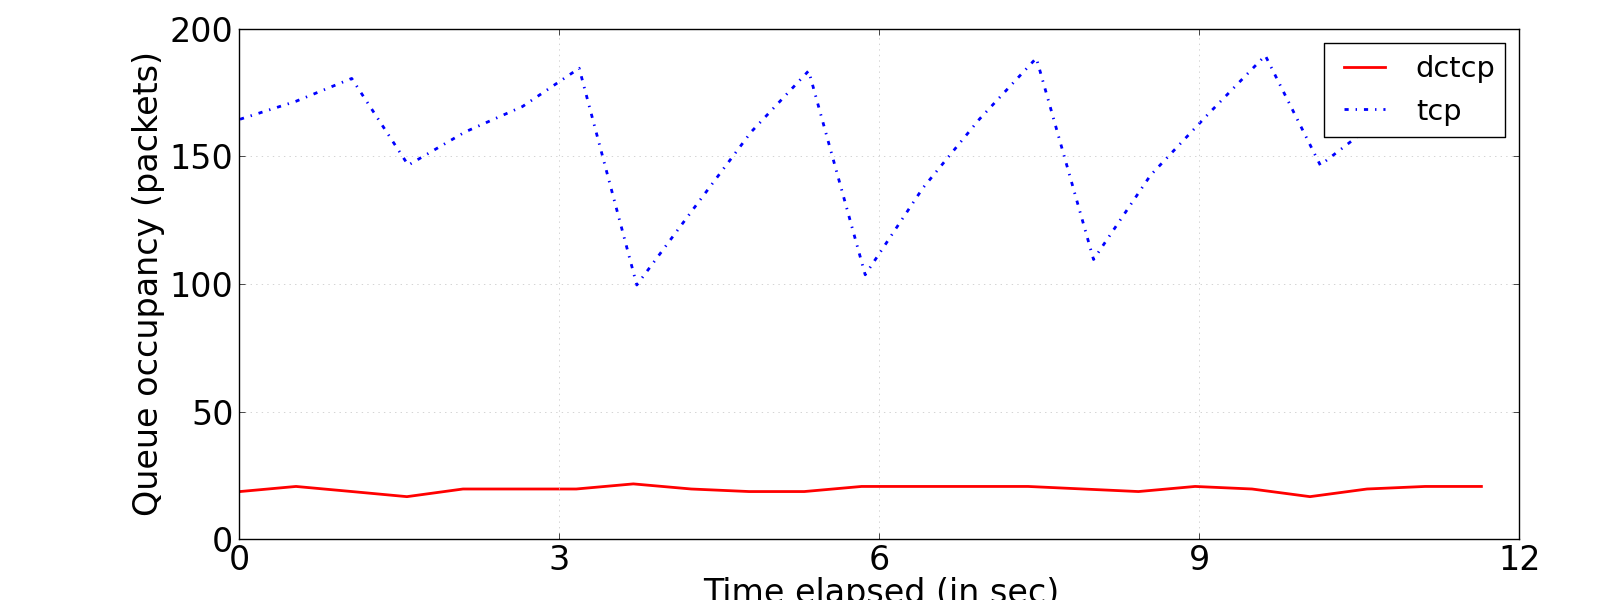
\includegraphics[scale=0.3]{imagens/dctcp_tcp_queue.png}
	    \end{figure}
	        
	
	    
	\end{frame}  


	
	\begin{frame} {Deadline-Agnostic: \textit{MPTCP}}
	                
	
	    \Large
	    \begin{itemize}
	                           
	        \item
	            Aproveita a existência de múltiplos caminhos na camada de agregação e na camada de núcleo        
	            No switch, quando a ocupância da fila ultrapassa o limiar K, marca os pacotes.
	        \item
	            Divide cada fluxo fonte-destino em subfluxos e usa o algoritmo de roteamento de múltiplos caminhos (ECMP).
	        \item
	            Apesar de melhorar a taxa de transferência, pode piorar o problema do incast.
	
	    \end{itemize}
	  
	\end{frame}
	  
	\begin{frame} {Deadline-Agnostic: \textit{MPTCP}}
	    
	    \Large
	    \begin{itemize}
	                           
	    \item
	      Inclui os subfluxos na pilha do protocolo, na camada de transporte.
	  
	    \begin{figure}[ht]    
	        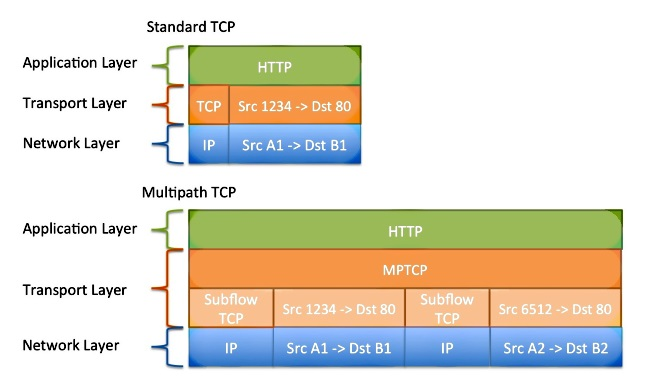
\includegraphics[scale=0.5]{imagens/mptcp_subfluxo.jpg}
	    \end{figure}
	        
	  \end{itemize}
	    
	\end{frame}  

	
	
	\begin{frame} {Deadline-Agnostic: \textit{ICTCP}}
	                
	
	    \Large
	    \begin{itemize}
	                           
	        \item
	            Variante do TCP especializada em resolver o problema do incast.
	        \item
	            Previne a perda de pacote ao invés de reenviar  quando há perda.
	        \item
	            Receptor sabe a taxa de transferência e largura de banda disponível.
	
	    \end{itemize}
	  
	\end{frame}
	  
	
	\begin{frame} {Deadline-Agnostic: \textit{ICTCP}}
	                
	    \Large
	    \begin{itemize}
	    
	        \item
	            Receptor usa a largura de banda disponível como indicador para prevenir o incast.
	        \item
	            O intervalo do controle de congestionamento é ajustado para o RTT de cada fluxo.
	        \item
	            O tamanho da janela de congestionamento deve levar em conta o estado de congestionamento e o requisitado pela aplicação.
	        \item
	            Basicamente, o tamanho da janela de congestionamento é ajustado para cada conexão, estimando a largura de banda disponível e o RTT.
	    \end{itemize}
	  
	\end{frame}
	
	\begin{frame} {Deadline-Agnostic: \textit{ICTCP}}
	    
	    \Large
	    \begin{itemize}
	                           
	    \item
	      Precisa ser implementado na pilha do TCP
	  
	    \begin{figure}[ht]    
	        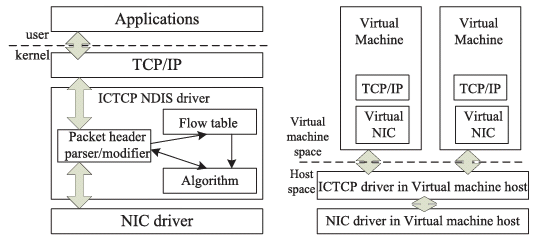
\includegraphics[scale=0.7]{imagens/ictcp_pilha.png}
	    \end{figure}
	        
	  \end{itemize}
	    
	\end{frame}  


    \begin{frame} {Deadline-Aware: $D^3$}
		\begin{itemize}
		 	\item
		 		Recebe a informação do tamanho do fluxo e o deadline
		 	\item
				Algoritmo guloso para tentar cumprir o máximo de deadlines possíveis
		 	\item
				Roteadores tentam alocar uma taxa adequada para cada fluxo
		 	\item
				Emissor envia dados com a mínima taxa alocada no próximo RTT
		 	\item
				A fonte periodicamente requisita uma nova taxa baseada no deadline e o tamanho do fluxo restante
		 \end{itemize}
	\end{frame}

	\begin{frame} {Deadline-Aware: $D^3$}
		\begin{itemize}
		 	\item
		 		Switches precisam de modificações para lidar com as requisições
		 	\item
				Não é compatível com o TCP tradicional, por causa da alocação de largura banda baseado em prioridades sem a informação do deadline no header
		 	\item
				Alocação com algoritmo guloso pode alocar largura de banda para fluxos com deadlines distantes ao invés de deadlines próximos, o que pode causar maior perda de deadlines
		 	\item
				Requisições constantes de taxas tem um overhead
		 \end{itemize}
	\end{frame}

	\begin{frame} {Deadline-Aware: $D^2TCP$}
		\begin{itemize}
		 	\item
		 		Baseado no DCTCP, mas leva o deadline em consideração para redimensionar a janela de congestionamento
		 	\item
				Se a maioria dos deadlines são próximos, ainda pode ocorrer congestionamento
		 	\item
				Se a maioria dos deadlines são distantes, ocorrerá a sub-utilização da rede e baixa taxa de transferência
		 	\item
				Se todos os deadlines são próximos, estão competindo pela largura de banda e nenhum fluxo é adiado, todos os deadlines não serão cumpridos. Caso um fluxo seja adiado, todos os outros podem ser cumpridos.
		 	\item
				O problema é saber qual fluxo sacrificar para satisfazer o máximo de deadlines possíveis
		 \end{itemize}
	\end{frame}

	\begin{frame} {Deadline-Aware: $DeTail$}
		\begin{itemize}
		 	\item
		 		Fluxos são associados com prioridades e os switches usam filas de prioridades nas portas de saída e de entrada
		 	\item
				Cada camada da abstração da rede tem uma função
		 \end{itemize}

		\begin{figure}[ht]   
			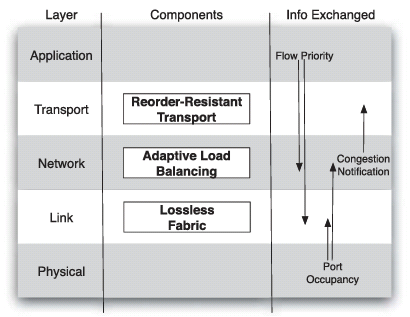
\includegraphics[scale=0.5]{imagens/detail.png}
			\label{fig:sample_figure}
		\end{figure}
	\end{frame}

	\begin{frame} {Deadline-Aware: $DeTail$}
		Enlace:
		\begin{itemize}
		 	\item
		 		Controle de fluxo “hop-by-hop” 
		 	\item
				Tenta amenizar o bloqueio de “head-of-line” (HOL)
		 	\item
				Recebe informações da camada de rede em relação ao balanco de carga adaptativo
		 	\item
				Recebe informações da camada de transporte sobre o estado do ECN
		 \end{itemize}
	\end{frame}

	\begin{frame} {Deadline-Aware: $DeTail$}
		Rede:
		\begin{itemize}
		 	\item
		 		Balanço de carga adaptativo baseado em pacotes de acordo com o nível de congestionamento
		 	\item
				Pode transmitir pacotes por caminhos que estão com pouca carga
		 \end{itemize}
	\end{frame}

	\begin{frame} {Deadline-Aware: $DeTail$}
		Transporte:
		\begin{itemize}
		 	\item
		 		Usa o ECN para marcar fluxos de baixa prioridade quando os bytes transmitidos para o destino ultrapassam um certo limiar
		 	\item
				Previne congestionamento persistente
		 \end{itemize}
	\end{frame}

	\begin{frame} {Deadline-Aware: $DeTail$}
		Aplicação:
		\begin{itemize}
		 	\item
		 		Seleciona as prioridades de cada fluxo baseado na sensibilidade de latência
		 \end{itemize}
	\end{frame}

	\begin{frame} {Deadline-Aware: $PDQ$}
		\begin{itemize}
		 	\item
		 		Semelhante ao $D^3$, mas ao contrário do $D^3$, escalona taxas de acordo com a criticalidade dos fluxos ao invés da política “first-come first-serve”
		 	\item
		 		Duas políticas de alocação, implementadas de forma totalmente distribuída:
				\begin{itemize}
				 	\item
				 		EDF (Earliest Deadline First)
				 	\item
						SJF (Shortest Job First)
				 \end{itemize}
		\end{itemize}
	\end{frame}


\section{Tendências}
    \begin{frame} {Facebook Fabric}
	  \begin{itemize}        
		            \item
		                  A próxima geração de data center do Facebook
		             \item
		               Topologia não hierarquizada
		                
		               \item
		                 Rede de alto desempenho
		               \item
		               		Sem oversubscription
		     \end{itemize}
              \begin{columns}    
                \column{0.5\textwidth}   
              \begin{figure}[ht]    
                  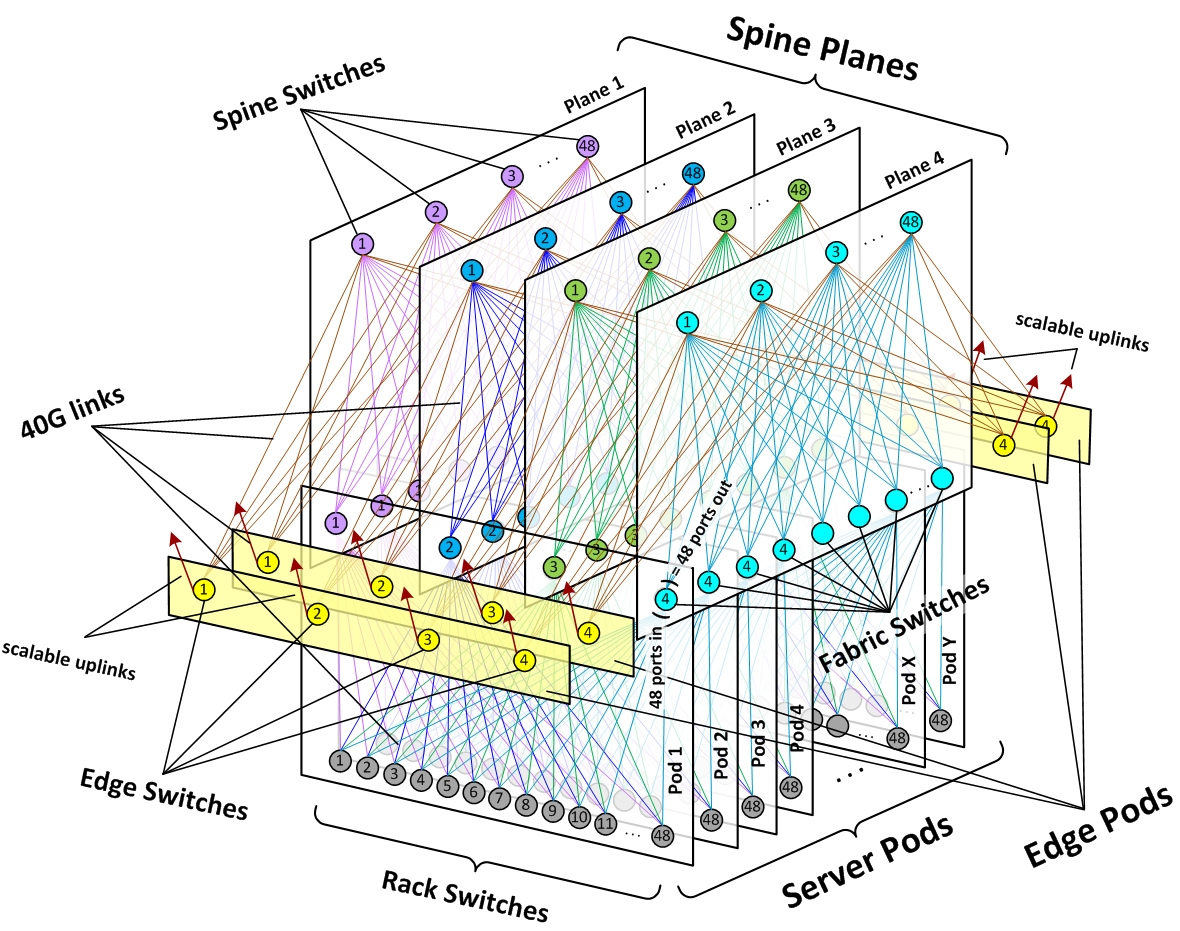
\includegraphics[scale=0.3]{scheme_fabric.jpg}
                  \label{fig:problems}
              \end{figure}
                         
             \column{0.5\textwidth}   
             \begin{figure}[ht]    
                             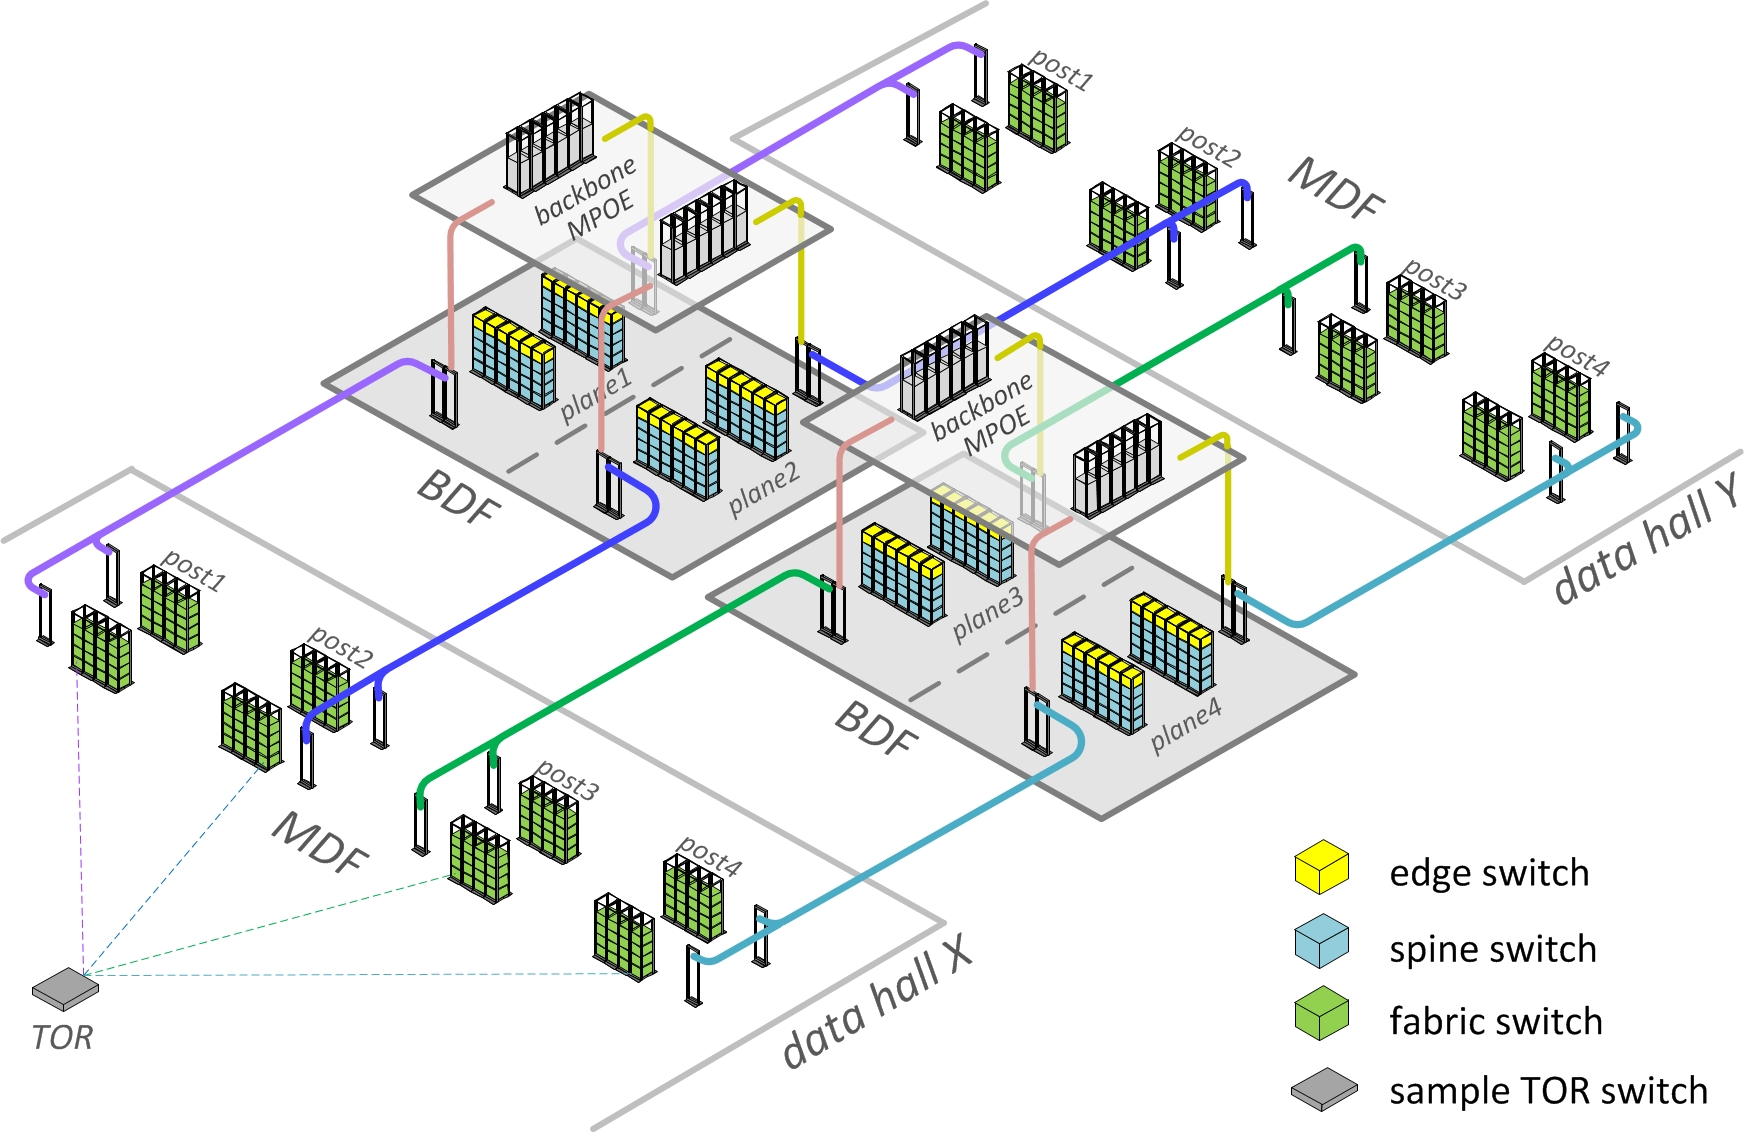
\includegraphics[scale=0.23]{phisic_fabric.jpg}
                             \label{fig:problems}
                         \end{figure}
            \end{columns}
    \end{frame}

	\begin{frame} {Next-Generation Technologies}
		SDDC (Software Defined Data Center): Com o avanço do SDN e virtualização de recursos, a tendência é montar data centers sob demanda. Estes data centers definidos por software são independentes da topologia e possuem um gerenciador de recursos fazendo a interface entre a rede física e a rede virtualizada.
	\end{frame}

	\begin{frame} {Next-Generation Technologies}
		DCOS (Data Center Operational System): Responsável por gerenciar os recursos físicos, fazendo a interface com os recursos virtualizados, o gerenciamento de usuários e máquinas virtuais.
	\end{frame}

	\begin{frame} {Next-Generation Technologies}
		Independente de infraestrutura: Um requisito para os data centers da próxima geração é a independência da infraestrutura, ou seja, não importa qual plataforma, camada de armazenamento ou supervisor sejam usados, o controlador deve saber escalonar recursos de forma eficiente.
	\end{frame}

\section{Conclusão}
    \begin{frame} 
        \begin{itemize}
			\item
				Data centers atualmente possuem um papel muito importante, uma vez que conseguem disponibilizar informações de modo rápido e em qualquer lugar.
			\item
				Oferecem serviços de processamento e armazenamento para grandes empresas, sem que haja necessidade de obter um infraestrutura própria.
			\item
				A tendência é que a indústria invista cada vez mais em P\&D na estrutura e comunicação de data centers. Uma vez que, a demanda dos usuários cresce exponencialmente.
		\end{itemize}
    \end{frame}
        
\section{Pergunta}
    \begin{frame} 
        As redes de datacenters possuem certos requisitos relacionados ao desempenho da rede. Cite 2 desses requisitos e explique como eles afetam o desempenho.\\ 
\hfill \break
		Referência: \\
		Rethinking the Data Center Networking: Architecture, Network Protocols and Resource Sharing\\
\hfill \break
		Ting Wang, Zhiyang Su, Yu Xia and Mounir Hamdi\\
\hfill \break
		\href{http://ieeexplore.ieee.org/stamp/stamp.jsp?tp=\&arnumber=6990724}{http://ieeexplore.ieee.org/stamp/stamp.jsp?tp=\&arnumber=6990724}
    \end{frame}
    
\end{document}
